\chapter{Аналитическая часть}

\section{Аппроксимация функций}

Под \textbf{аппроксимацией} понимается некоторое \textbf{приближение}, приближенное
представление. Соответственно, если речь идёт об аппроксимации функции, то ставится
вопрос о её замене другой, например, более простой функцией, которая в каком-то смысле
близка к заданной. В результате строится система
алгебраических уравнений, аппроксимирующих исходную дифференциальную задачу.

По сути, речь идёт о восстановлении непрерывной функции по заданному набору её значений для непрерывного множества значений аргумента. Так, исходную функциональную зависимость $y(x)$, заменяют приближенной функцией $\phi(x, \overline{a})$, которую и
используют в дальнейших вычислениях. При этом близость $y(x)$ и $\phi(x, \overline{a})$ обеспечивается подбором свободных параметров $\overline{a}={a_0, a_1, \dots, a_m}$ в соответствии с
некоторым критерием, определяющим степень совпадения аппроксимируемой и
аппроксимирующей функций. В данной работе в качестве такого критерия предлагается использовать среднеквадратичное отклонение

\label{deviation}
\begin{equation}
	\sigma^2 = \frac{1}{n}\sum_{i=1}^{n} (y(x_i) - \phi(x_i, \overline{a}))^2.
\end{equation}

При этом функция $\phi(x_i, \overline{a})$ определяется следующим образом.

\label{phi}
\begin{equation}
	\phi(x_i, \overline{a}) = \sum_{k=0}^{m} a_k x_i^k.
\end{equation}

Для аппроксимации функции $f(x) = sin(x)*(sin(x)+cos(x))$ предлагается взять полином 5 степени ($m = 5$), а для функции $g(x) = x^3 - x +3$ --- полином 3 степени ($m = 3$).

\section{Общие этапы функционирования системы}

Генетические и эволюционные  алгоритмы будут использоваться для подбора и оптимизации коэффициентов $\overline{a}$ полинома $\phi(x_i, \overline{a})$.

На рисунке \ref{img:algo} представлены основные этапы работы генетического алгоритма.~\cite{book1}

\begin{figure}
	\begin{center}
		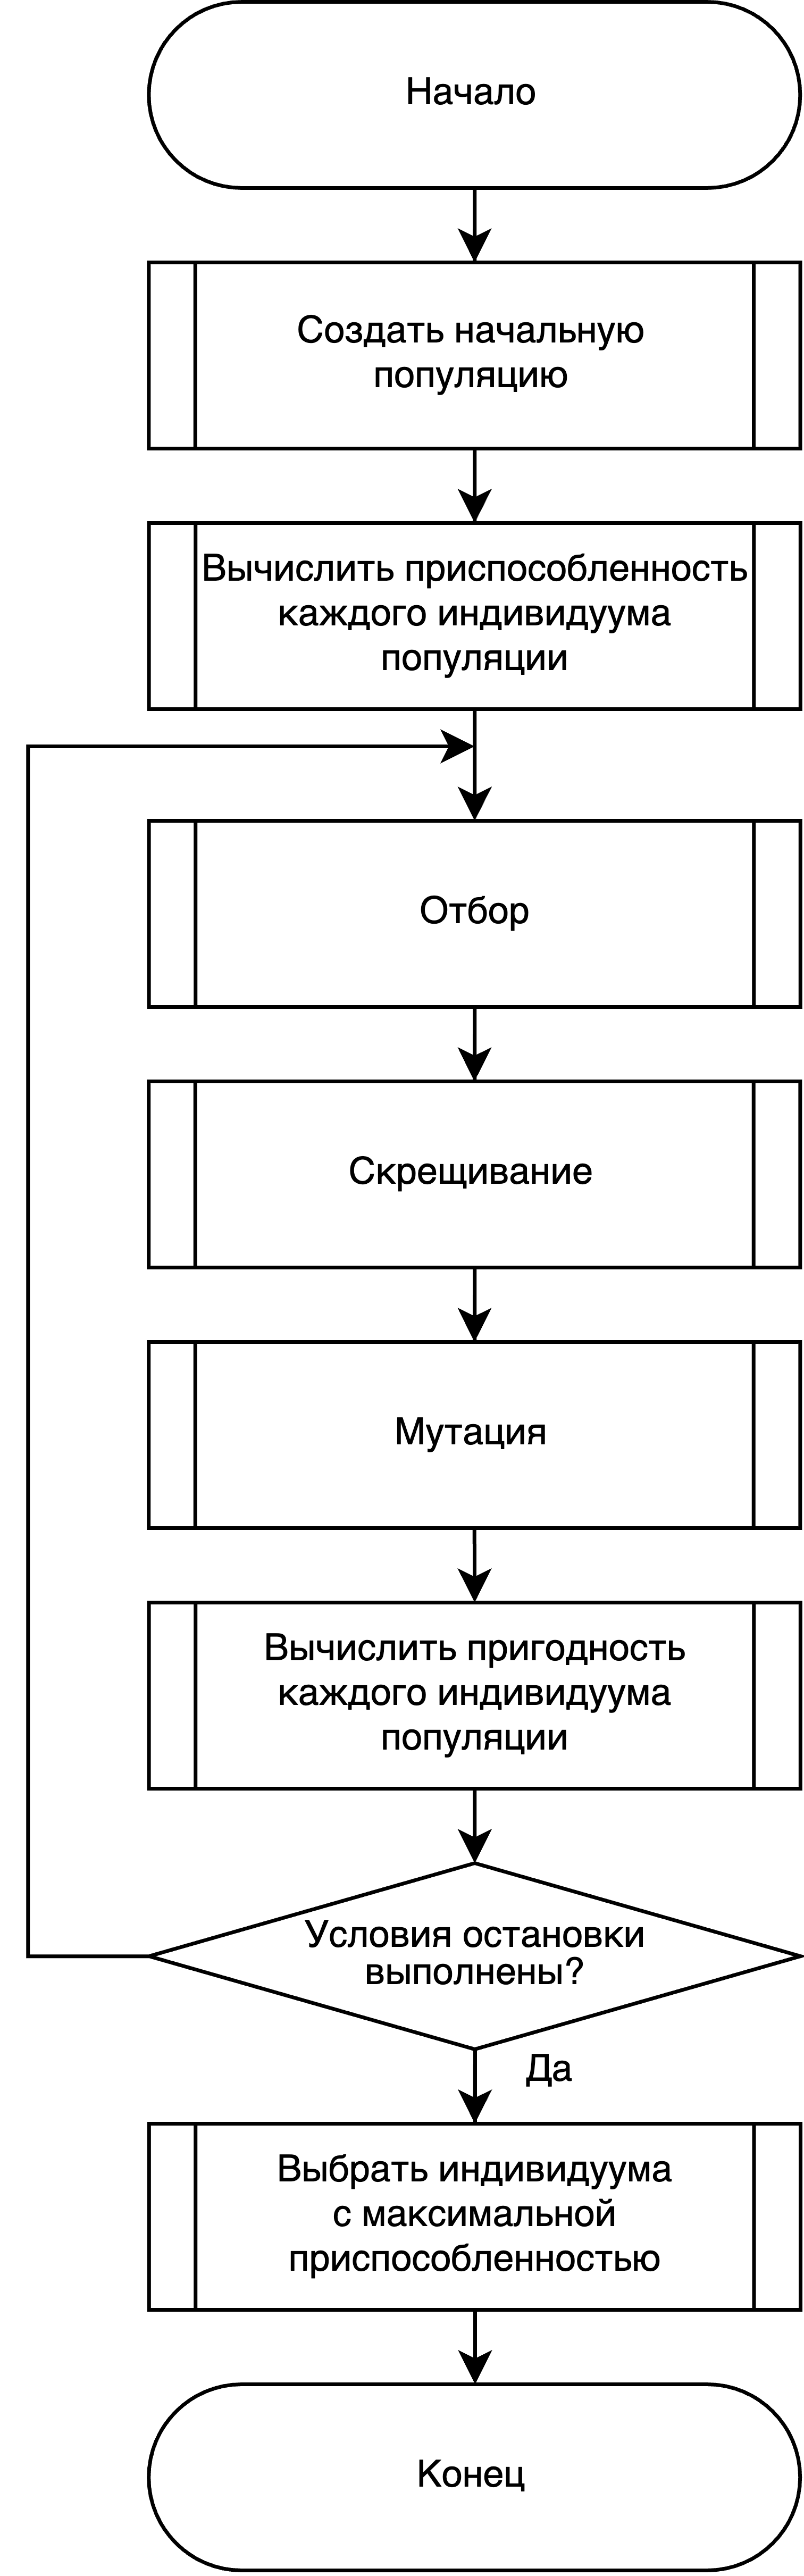
\includegraphics[height=0.95\textheight]{images/algo.png}
	\end{center}
	\caption{Основные этапы работы генетического алгоритма}
	\label{img:algo}
\end{figure}



\section*{Вывод}

В данном разделе были описаны общие этапы работы генетических алгоритмов.

\clearpage
